  %%%%%%%%%%%%%%%%%%%%%%%%%%%%%%%%%%%%%%%%%
% Classicthesis Typographic Thesis
% LaTeX Template
% Version 1.1 (4/8/12)
%
% This template has been downloaded from:
% http://www.LaTeXTemplates.com
%
% Original author:
% André Miede (http://www.miede.de)
%
% License:
% CC BY-NC-SA 3.0 (http://creativecommons.org/licenses/by-nc-sa/3.0/)
%
% General Tips:
% 1) Make sure to edit the classicthesis-config.file
% 2) New enumeration (A., B., C., etc in small caps): \begin{aenumerate} \end{aenumerate}
% 3) For margin notes: \marginpar or \graffito{}
% 4) Do not use bold fonts in this style, it is designed around them
% 5) Use tables as in the examples
% 6) See classicthesis-preamble.sty for useful commands
%
%%%%%%%%%%%%%%%%%%%%%%%%%%%%%%%%%%%%%%%%%

%----------------------------------------------------------------------------------------
%	PACKAGES AND OTHER DOCUMENT CONFIGURATIONS
%----------------------------------------------------------------------------------------

\documentclass[
		twoside,openright,titlepage,numbers=noenddot,headinclude,%1headlines,
                footinclude=true,cleardoublepage=empty,
                BCOR=5mm,paper=a4,fontsize=11pt, % Binding correction, paper type and font size
                ngerman,american, % Languages
                ]{scrreprt} 
                
% Includes the file which contains all the document configurations and packages - make sure to edit this file
%%%%%%%%%%%%%%%%%%%%%%%%%%%%%%%%%%%%%%%%%
% Thesis Configuration File
%
% The main lines to change in this file are in the DOCUMENT VARIABLES
% section, the rest of the file is for advanced configuration.
%
%%%%%%%%%%%%%%%%%%%%%%%%%%%%%%%%%%%%%%%%%

%----------------------------------------------------------------------------------------
%	DOCUMENT VARIABLES
%	Fill in the lines below to enter your information into the thesis template
%	Each of the commands can be cited anywhere in the thesis
%----------------------------------------------------------------------------------------

% Remove drafting to get rid of the '[ Date - classicthesis version 4.0 ]' text at the bottom of every page
\PassOptionsToPackage{eulerchapternumbers,listings,drafting, pdfspacing, subfig,beramono,eulermath,parts}{classicthesis}
% Available options: drafting parts nochapters linedheaders eulerchapternumbers beramono eulermath pdfspacing minionprospacing tocaligned dottedtoc manychapters listings floatperchapter subfig
% Adding 'dottedtoc' will make page numbers in the table of contents flushed right with dots leading to them

\newcommand{\myTitle}{A Classic Thesis Style\xspace}
\newcommand{\mySubtitle}{An Homage to The Elements of Typographic Style\xspace}
\newcommand{\myDegree}{Doktor-Ingenieur (Dr.-Ing.)\xspace}
\newcommand{\myName}{Andr\'e Miede\xspace}
\newcommand{\myProf}{Put name here\xspace}
\newcommand{\myOtherProf}{Put name here\xspace}
\newcommand{\mySupervisor}{Put name here\xspace}
\newcommand{\myFaculty}{Put data here\xspace}
\newcommand{\myDepartment}{Put data here\xspace}
\newcommand{\myUni}{Put data here\xspace}
\newcommand{\myLocation}{Darmstadt\xspace}
\newcommand{\myTime}{December 2011\xspace}
\newcommand{\myVersion}{version 4.0\xspace}

%----------------------------------------------------------------------------------------
%	USEFUL COMMANDS
%----------------------------------------------------------------------------------------

\newcommand{\ie}{i.\,e.}
\newcommand{\Ie}{I.\,e.}
\newcommand{\eg}{e.\,g.}
\newcommand{\Eg}{E.\,g.} 

\newcounter{dummy} % Necessary for correct hyperlinks (to index, bib, etc.)
\providecommand{\mLyX}{L\kern-.1667em\lower.25em\hbox{Y}\kern-.125emX\@}

%----------------------------------------------------------------------------------------
%	PACKAGES
%----------------------------------------------------------------------------------------

\usepackage{lipsum} % Used for inserting dummy 'Lorem ipsum' text into the template

%------------------------------------------------
 
\PassOptionsToPackage{latin9}{inputenc} % latin9 (ISO-8859-9) = latin1+"Euro sign"
\usepackage{inputenc}
 
 %------------------------------------------------

%\PassOptionsToPackage{ngerman,american}{babel}  % Change this to your language(s)
% Spanish languages need extra options in order to work with this template
%\PassOptionsToPackage{spanish,es-lcroman}{babel}
\usepackage{babel}

%------------------------------------------------			

\PassOptionsToPackage{square,numbers}{natbib}
 \usepackage{natbib}
 
 %------------------------------------------------

\PassOptionsToPackage{fleqn}{amsmath} % Math environments and more by the AMS 
 \usepackage{amsmath}
 
 %------------------------------------------------

\PassOptionsToPackage{T1}{fontenc} % T2A for cyrillics
\usepackage{fontenc}

%------------------------------------------------

\usepackage{xspace} % To get the spacing after macros right

%------------------------------------------------

\usepackage{mparhack} % To get marginpar right

%------------------------------------------------

\usepackage{fixltx2e} % Fixes some LaTeX stuff 

%------------------------------------------------

\PassOptionsToPackage{smaller}{acronym} % Include printonlyused in the first bracket to only show acronyms used in the text
\usepackage{acronym} % nice macros for handling all acronyms in the thesis

%------------------------------------------------

%\renewcommand*{\acsfont}[1]{\textssc{#1}} % For MinionPro
\renewcommand{\bflabel}[1]{{#1}\hfill} % Fix the list of acronyms

%------------------------------------------------

\PassOptionsToPackage{pdftex}{graphicx}
\usepackage{graphicx} 

%----------------------------------------------------------------------------------------
%	FLOATS: TABLES, FIGURES AND CAPTIONS SETUP
%----------------------------------------------------------------------------------------

\usepackage{tabularx} % Better tables
\setlength{\extrarowheight}{3pt} % Increase table row height
\newcommand{\tableheadline}[1]{\multicolumn{1}{c}{\spacedlowsmallcaps{#1}}}
\newcommand{\myfloatalign}{\centering} % To be used with each float for alignment
\usepackage{caption}
\captionsetup{format=hang,font=small}
\usepackage{subfig}  

%----------------------------------------------------------------------------------------
%	CODE LISTINGS SETUP
%----------------------------------------------------------------------------------------

\usepackage{listings} 
%\lstset{emph={trueIndex,root},emphstyle=\color{BlueViolet}}%\underbar} % for special keywords
\lstset{language=[LaTeX]Tex, % Specify the language for listings here
keywordstyle=\color{RoyalBlue}, % Add \bfseries for bold
basicstyle=\small\ttfamily, % Makes listings a smaller font size and a different font
%identifierstyle=\color{NavyBlue}, % Color of text inside brackets
commentstyle=\color{Green}\ttfamily, % Color of comments
stringstyle=\rmfamily, % Font type to use for strings
numbers=left, % Change left to none to remove line numbers
numberstyle=\scriptsize, % Font size of the line numbers
stepnumber=5, % Increment of line numbers
numbersep=8pt, % Distance of line numbers from code listing
showstringspaces=false, % Sets whether spaces in strings should appear underlined
breaklines=true, % Force the code to stay in the confines of the listing box
%frameround=ftff, % Uncomment for rounded frame
frame=single, % Frame border - none/leftline/topline/bottomline/lines/single/shadowbox/L
belowcaptionskip=.75\baselineskip % Space after the "Listing #: Desciption" text and the listing box
}

%----------------------------------------------------------------------------------------
%	HYPERREFERENCES
%----------------------------------------------------------------------------------------

\PassOptionsToPackage{pdftex,hyperfootnotes=false,pdfpagelabels}{hyperref}
\usepackage{hyperref}  % backref linktocpage pagebackref
\pdfcompresslevel=9
\pdfadjustspacing=1

\hypersetup{
% Uncomment the line below to remove all links (to references, figures, tables, etc)
%draft, 
colorlinks=true, linktocpage=true, pdfstartpage=3, pdfstartview=FitV,
% Uncomment the line below if you want to have black links (e.g. for printing black and white)
%colorlinks=false, linktocpage=false, pdfborder={0 0 0}, pdfstartpage=3, pdfstartview=FitV, 
breaklinks=true, pdfpagemode=UseNone, pageanchor=true, pdfpagemode=UseOutlines,
plainpages=false, bookmarksnumbered, bookmarksopen=true, bookmarksopenlevel=1,
hypertexnames=true, pdfhighlight=/O, urlcolor=webbrown, linkcolor=RoyalBlue, citecolor=webgreen,
%------------------------------------------------
% PDF file meta-information
pdftitle={\myTitle},
pdfauthor={\textcopyright\ \myName, \myUni, \myFaculty},
pdfsubject={},
pdfkeywords={},
pdfcreator={pdfLaTeX},
pdfproducer={LaTeX with hyperref and classicthesis}
%------------------------------------------------
}   

%----------------------------------------------------------------------------------------
%	BACKREFERENCES
%----------------------------------------------------------------------------------------

\usepackage{ifthen} % Allows the user of the \ifthenelse command
\newboolean{enable-backrefs} % Variable to enable backrefs in the bibliography
\setboolean{enable-backrefs}{false} % Variable value: true or false

\newcommand{\backrefnotcitedstring}{\relax} % (Not cited.)
\newcommand{\backrefcitedsinglestring}[1]{(Cited on page~#1.)}
\newcommand{\backrefcitedmultistring}[1]{(Cited on pages~#1.)}
\ifthenelse{\boolean{enable-backrefs}} % If backrefs were enabled
{
\PassOptionsToPackage{hyperpageref}{backref}
\usepackage{backref} % to be loaded after hyperref package 
\renewcommand{\backreftwosep}{ and~} % separate 2 pages
\renewcommand{\backreflastsep}{, and~} % separate last of longer list
\renewcommand*{\backref}[1]{}  % disable standard
\renewcommand*{\backrefalt}[4]{% detailed backref
\ifcase #1 
\backrefnotcitedstring
\or
\backrefcitedsinglestring{#2}
\else
\backrefcitedmultistring{#2}
\fi}
}{\relax} 

%----------------------------------------------------------------------------------------
%	AUTOREFERENCES SETUP
%	Redefines how references in text are prefaced for different 
%	languages (e.g. "Section 1.2" or "section 1.2")
%----------------------------------------------------------------------------------------

\makeatletter
\@ifpackageloaded{babel}
{
\addto\extrasamerican{
\renewcommand*{\figureautorefname}{Figure}
\renewcommand*{\tableautorefname}{Table}
\renewcommand*{\partautorefname}{Part}
\renewcommand*{\chapterautorefname}{Chapter}
\renewcommand*{\sectionautorefname}{Section}
\renewcommand*{\subsectionautorefname}{Section}
\renewcommand*{\subsubsectionautorefname}{Section}
}
\addto\extrasngerman{
\renewcommand*{\paragraphautorefname}{Absatz}
\renewcommand*{\subparagraphautorefname}{Unterabsatz}
\renewcommand*{\footnoteautorefname}{Fu\"snote}
\renewcommand*{\FancyVerbLineautorefname}{Zeile}
\renewcommand*{\theoremautorefname}{Theorem}
\renewcommand*{\appendixautorefname}{Anhang}
\renewcommand*{\equationautorefname}{Gleichung}
\renewcommand*{\itemautorefname}{Punkt}
}
\providecommand{\subfigureautorefname}{\figureautorefname} % Fix to getting autorefs for subfigures right
}{\relax}
\makeatother

%----------------------------------------------------------------------------------------

\usepackage{classicthesis} 

%----------------------------------------------------------------------------------------
%	CHANGING TEXT AREA 
%----------------------------------------------------------------------------------------

%\linespread{1.05} % a bit more for Palatino
%\areaset[current]{312pt}{761pt} % 686 (factor 2.2) + 33 head + 42 head \the\footskip
%\setlength{\marginparwidth}{7em}%
%\setlength{\marginparsep}{2em}%

%----------------------------------------------------------------------------------------
%	USING DIFFERENT FONTS
%----------------------------------------------------------------------------------------

%\usepackage[oldstylenums]{kpfonts} % oldstyle notextcomp
%\usepackage[osf]{libertine}
%\usepackage{hfoldsty} % Computer Modern with osf
%\usepackage[light,condensed,math]{iwona}
%\renewcommand{\sfdefault}{iwona}
%\usepackage{lmodern} % <-- no osf support :-(
%\usepackage[urw-garamond]{mathdesign} <-- no osf support :-(

\begin{document}

\frenchspacing % Reduces space after periods to make text more compact

\raggedbottom % Makes all pages the height of the text on that page

\selectlanguage{american} % Select your default language - e.g. american or ngerman

%\renewcommand*{\bibname}{new name} % Uncomment to change the name of the bibliography
%\setbibpreamble{} % Uncomment to include a preamble to the bibliography - some text before the reference list starts

\pagenumbering{roman} % Roman page numbering prior to the start of the thesis content (i, ii, iii, etc)

\pagestyle{plain} % Suppress headers for the pre-content pages

%----------------------------------------------------------------------------------------
%	PRE-CONTENT THESIS PAGES
%----------------------------------------------------------------------------------------

\pagestyle{scrheadings} % Show chapter titles as headings

\pagenumbering{arabic} % Arabic page numbering for thesis content (1, 2, 3, etc)
%\setcounter{page}{90} % Uncomment to manually start the page counter at an arbitrary value (for example if you wish to count the pre-content pages in the page count)

%----------------------------------------------------------------------------------------
%	THESIS CONTENT - CHAPTERS
%----------------------------------------------------------------------------------------

% \ctparttext{You can put some informational part preamble text here. Illo principalmente su nos. Non message \emph{occidental} angloromanic da. Debitas effortio simplificate sia se, auxiliar summarios da que, se avantiate publicationes via. Pan in terra summarios, capital interlingua se que. Al via multo esser specimen, campo responder que da. Le usate medical addresses pro, europa origine sanctificate nos se.} % Text on the Part 1 page describing  the content in Part 1

% \part{Some Kind of Manual} % First part of the thesis

% % Chapter 1

\chapter{Introduction} % Chapter title

\label{ch:introduction} % For referencing the chapter elsewhere, use \autoref{ch:introduction} 

%----------------------------------------------------------------------------------------

This template for \LaTeX\ has two goals:
\begin{enumerate}
\item Provide students with an easy-to-use template for their Master's or PhD thesis (though it might also be used by other types of authors for reports, books, etc.).
\item Provide a classic, high-quality typographic style that is inspired by \citeauthor{bringhurst:2002}'s ``\emph{The Elements of Typographic Style}'' \citep{bringhurst:2002}.
\marginpar{\myTitle \myVersion}
\end{enumerate}

The bundle is configured to run with a \emph{full} MiK\TeX\ or \TeX Live installation right away and, therefore, it uses only freely available fonts.

People interested only in the nice style and not the whole bundle can now use the style stand-alone via the file \texttt{classicthesis.sty}. This works now also with ``plain'' \LaTeX.

As of version 3.0, \texttt{classicthesis} can also be easily used with \mLyX\footnote{\url{http://www.lyx.org}} thanks to Nicholas Mariette and Ivo Pletikosi\'c. The \mLyX\ version of this manual will contain more information on the details.

This should enable anyone with a basic knowledge of \LaTeXe\ or \mLyX\ to produce beautiful documents without too much effort. In the end, this is my overall goal: more beautiful documents, especially theses, as I am tired of seeing so many ugly ones.

The whole template and the used style is released under the \textsmaller{GNU} General Public License. 

If you like the style then I would appreciate a postcard:
\begin{center}
Andre Miede \\
Detmolder Strasse 32 \\
31737 Rinteln \\
Germany
\end{center}

\noindent The postcards I received so far are available at:
\begin{center}
 \url{http://postcards.miede.de}
\end{center}
\marginpar{A well-balanced line width improves the legibility of the text. That's what typography is all about, right?} So far, many theses, some books, and several other publications have been typeset successfully with it. If you are interested in some typographic details behind it, enjoy Robert Bringhurst's wonderful book. % \citep{bringhurst:2002}.

\paragraph{Important Note:} Some things of this style might look unusual at first glance, many people feel so in the beginning. However, all things are intentionally designed to be as they are, especially these:
\begin{itemize}
\item No bold fonts are used. Italics or spaced small caps do the job quite well.
\item The size of the text body is intentionally shaped like it is. It supports both legibility and allows a reasonable amount of information to be on a page. And, no: the lines are not too short.
\item The tables intentionally do not use vertical or double rules. See the documentation for the \texttt{booktabs} package for a nice discussion of this topic.\footnote{To be found online at \\ \url{http://www.ctan.org/tex-archive/macros/latex/contrib/booktabs/}.}
\item And last but not least, to provide the reader with a way easier access to page numbers in the table of contents, the page numbers are right behind the titles. Yes, they are \emph{not} neatly aligned at the right side and they are \emph{not} connected with dots that help the eye to bridge a distance that is not necessary. If you are still not convinced: is your reader interested in the page number or does she want to sum the numbers up?
\end{itemize}

\noindent Therefore, please do not break the beauty of the style by changing these things unless you really know what you are doing! Please.

%----------------------------------------------------------------------------------------

\section{Organization}
A very important factor for successful thesis writing is the organization of the material. This template suggests a structure as the following:
\begin{itemize}
\marginpar{You can use these margins for summaries of the text body\dots}
\item\texttt{Chapters/} is where all the ``real'' content goes in separate files such as \texttt{Chapter01.tex} etc.
\item\texttt{FrontBackMatter/} is where all the stuff goes that surrounds the ``real'' content, such as the acknowledgments, dedication, etc.
\item\texttt{gfx/} is where you put all the graphics you use in the thesis. Maybe they should be organized into subfolders depending on the chapter they are used in, if you have a lot of graphics.
\item\texttt{Bibliography.bib}: the Bib\TeX\ database to organize all the references you might want to cite.
\item\texttt{classicthesis.sty}: the style definition to get this awesome look and feel. Bonus: works with both \LaTeX\ and \textsc{pdf}\LaTeX\dots and \mLyX.
\item\texttt{ClassicThesis.tcp} a \TeX nicCenter project file. Great tool and it's free!
\item\texttt{ClassicThesis.tex}: the main file of your thesis where all the content gets bundled together.
\item\texttt{classicthesis-config.tex}: a central place to load all nifty packages that are used. In there, you can also activate backrefs in order to have information in the bibliography about where a source was cited in the text (\ie, the page number).
    
\emph{Make your changes and adjustments here.} This means that you specify here the options you want to load \texttt{classicthesis.sty} with. You also adjust the title of your thesis, your name, and all similar information here. Refer to \autoref{sec:custom} for more information.

This had to change as of version 3.0 in order to enable an easy transition from the ``basic'' style to \mLyX.
\end{itemize}

\noindent In total, this should get you started in no time.

%----------------------------------------------------------------------------------------

\section{Style Options}\label{sec:options}

There are a couple of options for \texttt{classicthesis.sty} that allow for a bit of freedom concerning the layout: \marginpar{\dots or your supervisor might use the margins for some comments of her own while reading.}
\begin{itemize}
\item General:
\begin{itemize}
\item\texttt{drafting}: prints the date and time at the bottom of each page, so you always know which version you are dealing with. Might come in handy not to give your Prof. that old draft.
\end{itemize}
	
\item Parts and Chapters:
\begin{itemize}
\item\texttt{parts}: if you use Part divisions for your document, you should choose this option. (Cannot be used together with \texttt{nochapters}.)

\item\texttt{nochapters}: allows to use the look-and-feel with classes that do not use chapters, \eg, for articles. Automatically turns off a couple of other options: \texttt{eulerchapternumbers}, \texttt{linedheaders}, \texttt{listsseparated}, and \texttt{parts}. 

\item\texttt{linedheaders}: changes the look of the chapter headings a bit by adding a horizontal line above the chapter title. The chapter number will also be moved to the top of the page, above the chapter title.
\end{itemize}

\item Typography:
\begin{itemize}
\item\texttt{eulerchapternumbers}: use figures from Hermann Zapf's Euler math font for the chapter numbers. By default, old style figures from the Palatino font are used.

\item\texttt{beramono}: loads Bera Mono as typewriter font. (Default setting is using the standard CM typewriter font.)
\item\texttt{eulermath}: loads the awesome Euler fonts for math. (Palatino is used as default font.)

\item\texttt{pdfspacing}: makes use of pdftex' letter spacing capabilities via the \texttt{microtype} package.\footnote{Use \texttt{microtype}'s \texttt{DVIoutput} option to generate DVI with pdftex.} This fixes some serious issues regarding math formul\ae\ etc. (\eg, ``\ss'') in headers. 

\item\texttt{minionprospacing}: uses the internal \texttt{textssc} command of the \texttt{MinionPro} package for letter spacing. This automatically enables the \texttt{minionpro} option and overrides the \texttt{pdfspacing} option.
\end{itemize}  

\item Table of Contents:
\begin{itemize}
\item\texttt{tocaligned}: aligns the whole table of contents on the left side. Some people like that, some don't.

\item\texttt{dottedtoc}: sets pagenumbers flushed right in the table of contents.

\item\texttt{manychapters}: if you need more than nine chapters for your document, you might not be happy with the spacing between the chapter number and the chapter title in the Table of Contents. This option allows for additional space in this context. However, it does not look as ``perfect'' if you use \verb|\parts| for structuring your document.
\end{itemize}

\item Floats:
\begin{itemize}
\item\texttt{listings}: loads the \texttt{listings} package (if not already done) and configures the List of Listings accordingly.
    
\item\texttt{floatperchapter}: activates numbering per chapter for all floats such as figures, tables, and listings (if used).	
    
\item\texttt{subfig}(\texttt{ure}): is passed to the \texttt{tocloft} package to enable compatibility with the \texttt{subfig}(\texttt{ure}) package. Use this option if you want use classicthesis with the \texttt{subfig} package.

\end{itemize}    

\end{itemize}

\noindent The best way to figure these options out is to try the different possibilities and see, what you and your supervisor like best.

In order to make things easier in general, \texttt{classicthesis-config.tex} contains some useful commands that might help you.

%----------------------------------------------------------------------------------------

\section{Customization}\label{sec:custom}

This section will give you some hints about how to adapt \texttt{classicthesis} to your needs.

The file \texttt{classicthesis.sty} contains the core functionality of the style and in most cases will be left intact, whereas the file \texttt{classic\-thesis-config.tex} is used for some common user customizations. 

The first customization you are about to make is to alter the document title, author name, and other thesis details. In order to do this, replace the data in the following lines of \texttt{classicthesis-config.tex:}\marginpar{Modifications in \texttt{classic\-thesis-config.tex}
}

\begin{lstlisting}[frame=lt]
\newcommand{\myTitle}{A Classic Thesis Style\xspace}
\newcommand{\mySubtitle}{An Homage to ...\xspace}
\newcommand{\myDegree}{Doktor-Ingenieur (Dr.-Ing.)\xspace}
\end{lstlisting}

Further customization can be made in \texttt{classicthesis-config.tex} by choosing the options to \texttt{classicthesis.sty} (see~\autoref{sec:options}) in a line that looks like this:

\begin{lstlisting}[frame=lt]
\PassOptionsToPackage{eulerchapternumbers,listings,drafting, pdfspacing, subfig,beramono,eulermath,parts}{classicthesis}

\end{lstlisting}

If you want to use backreferences from your citations to the pages they were cited on, change the following line from:
\begin{lstlisting}[breaklines=false,frame=lt]
\setboolean{enable-backrefs}{false}
\end{lstlisting}
to
\begin{lstlisting}[breaklines=false,frame=lt]
\setboolean{enable-backrefs}{true}
\end{lstlisting}

Many other customizations in \texttt{classicthesis-config.tex} are possible, but you should be careful making changes there, since some changes could cause errors.

Finally, changes can be made in the file \texttt{classicthesis.sty}, \marginpar{Modifications in \texttt{classicthesis.sty}} although this is mostly not designed for user customization. The main change that might be made here is the text-block size, for example, to get longer lines of text.

%----------------------------------------------------------------------------------------

\section{Issues}\label{sec:issues}
This section will list some information about problems using \texttt{classic\-thesis} in general or using it with other packages.

Beta versions of \texttt{classicthesis} can be found at the following Google code repository:
\begin{center}
\url{http://code.google.com/p/classicthesis/}
\end{center}

\noindent There, you can also post serious bugs and problems you encounter.

\subsection*{Compatibility with the \texttt{glossaries} Package}
If you want to use the \texttt{glossaries} package, take care of loading it with the following options:
\begin{verbatim}
\usepackage[style=long,nolist]{glossaries}
\end{verbatim}

\noindent Thanks to Sven Staehs for this information. 

\subsection*{Compatibility with the (Spanish) \texttt{babel} Package}
Spanish languages need an extra option in order to work with this template:
\begin{verbatim}
\usepackage[spanish,es-lcroman]{babel}
\end{verbatim}

\noindent Thanks to an unknown person for this information (via Google Code issue reporting). 

\subsection*{Compatibility with the \texttt{pdfsync} Package}
Using the \texttt{pdfsync} package leads to linebreaking problems with the \texttt{graffito} command. Thanks to Henrik Schumacher for this information. 

%----------------------------------------------------------------------------------------

\section{Future Work}
So far, this is a quite stable version that served a couple of people well during their thesis time. However, some things are still not as they should be. Proper documentation in the standard format is still missing. In the long run, the style should probably be published separately, with the template bundle being only an application of the style. Alas, there is no time for that at the moment\dots it could be a nice task for a small group of \LaTeX nicians.

Please do not send me email with questions concerning \LaTeX\ or the template, as I do not have time for an answer. But if you have comments, suggestions, or improvements for the style or the template in general, do not hesitate to write them on that postcard of yours.

%----------------------------------------------------------------------------------------

\section{License}
\paragraph{GNU General Public License:} This program is free software; you can redistribute it and/or modify it under the terms of the \textsmaller{GNU} General Public License as published by the Free Software Foundation; either version 2 of the License, or (at your option) any later version.

This program is distributed in the hope that it will be useful, but \emph{without any warranty}; without even the implied warranty of \emph{merchantability} or \emph{fitness for a particular purpose}. See the \textsmaller{GNU} General Public License for more details. % Chapter 1

% \cleardoublepage % Empty page before the start of the next part

%------------------------------------------------

\ctparttext{ML ML You can put some informational part preamble text here. Illo principalmente su nos. Non message \emph{occidental} angloromanic da. Debitas effortio simplificate sia se, auxiliar summarios da que, se avantiate publicationes via. Pan in terra summarios, capital interlingua se que. Al via multo esser specimen, campo responder que da. Le usate medical addresses pro, europa origine sanctificate nos se.} % Text on the Part 2 page describing the content in Part 2

% \part{The Showcase} % Second part of the thesis

% Chapter 2

\chapter{Constrained Inference - Zenna Tavares} % Chapter title

We address the problem of tractably drawing exact samples from conditional probability distributions.
In particular we propose a formalism for constructively incorporating constraints into generative models for probabilstic inference.
Building upon formalisms of inference as conditional execution of a program, we outline approaches to analyse and transform the formal semantics of a probabilstic program.

\section{Introduction}
\label{ch:examples} % For referencing the chapter elsewhere, use \autoref{ch:examples} 

%----------------------------------------------------------------------------------------

Probabilstic inference has established itself as a means of reasoning in domains subject to uncertainty.
Although the rules of conditional probability state how to update our beliefs in hypotheses conditioned on evidence, it tells us only declaratively, and leaves us with no guidance as to how hypotheses should be constructed in the first place.
In anticipation of the distinction emphasised in this essay, we describe conditional probability and in particular Bayes' Rule as the \textit{logic} of a program, while the the \textit{control} or \textit{procedure} remains a topic of continued research.

Inference typically refers to finding the expectation of some function with respect to a probability distribution, computing the posterior distribution, or drawing samples to approximate it.
Numerous approaches exist, but our focus is on Monte Carlo methods whose strengths lie in their applicability to high dimensional distributions, where direct sampling becomes intractable.
Inference by means of random perturbations to hypotheses is often inefficient however; we would prefer to not waste resources proposing candidate hypotheses which violate sensible constraints.
In other words, we would like to make good guesses.

The objective of this study is to explore conceptual and practical methods of making good guesses by incorporating constraints \textit{constructively} into generative models.
We frame construction in constrast to testing; to construct is (ideally) to not test.
\graffito{Universal inference \citep{church} is analagous to notions of universality in computation.  Informally it refers to the ability to perform conditional simulation of any computable probabilstic generative process.}
We build upon recent interpretations of probabilstic inference in computational terms, in particular the \spacedlowsmallcaps{query} operation, which performs universal inference in the probabilstic programming language Church \citep{church}.
We suggest a new constructive perspective \spacedlowsmallcaps{constrain}, which given a generative model manifested as a stochastic {\em prior program} $P$, and a conditioning predicate $C$ aims to construct a new program $P^*$ which samples only values which adhere to our condition.

The feasibility of this aim is vulnerable to skepticism; how can we construct only constrained proposals without testing to see if they satisfy our constraints?
It is unlikely this objective can be achieved in full generality, in some cases we have no alternative than to generate and test.
Furthermore we shall see that relaxations of the above maxim may lead to more pragmatic implementation strategies; to construct is to test less perhaps, or to test only partially and incrementally.
Precisely what distuiginshes one constraint from another in terms of the extent to which it can be implemented constructively, is a topic of great interest and speculated on in our conclusion.
Yet, we can motivate the plausiibilty of constructive inference by appealling to common experience:
consider the ease with one can compose a paragraph that rhymes, generate a polynomial expression, or draw an acyclic graph.
Each of these examples entails a logical constraint which we satisfy without hinderance.
While it is risky to draw conclusions about the computational hardness of a problem based on our subjective difficulty when solving it, each of the above examples has a known efficient algorithm.

% A further appeal of such as approach is its potential to bridge between discriminative and generative approaches
% Discriminative models may detect broad level characteristics of a scene, while generative use these as constraints.

First we will summarise \spacedlowsmallcaps{query}, a computational theory of probabilstic inference.
Then we formalise the key concept of this paper, \spacedlowsmallcaps{constrain}, in terms of \spacedlowsmallcaps{query}.
Two approaches to implementing \spacedlowsmallcaps{constrain} are then described in detail.
%----------------------------------------------------------------------------------------

\subsection{Query}

\spacedlowsmallcaps{query} formalises probabilistic inference as a \textit{program} in a corresponding model of computation.
Developed first as a primitive function in the probabilstic programming language Church \citep{church}, \spacedlowsmallcaps{query} has been described in terms of probabilstic generalisations of the $\lambda$-calculus and Turing machine, both classical models of computation.

In its original formulation, \spacedlowsmallcaps{query} is a higher order function which accepts as input a stochastic expression to be evaluated and a set of predicate conditions.
In lisp (clojure) notation:

\marginpar{Notation: defn defines a function.  The following term is the function name and terms inside square brackets [] are argument names.  \'Let\' is used to assign names to values, conceptually similar to assignment of values to variables in imperative languages.}
\begin{verbatim}
(defn query [exp pred]          ; Define function
  (let ((val (eval exp))        ; sample from model, call it val
    (if (pred val)              ; If val satisfies conditions
        val                     ; Then.. return it
        (query exp pred)))))    ; Otherwise try again
\end{verbatim}

In \citep{freer} a formulation in terms of a probalistic turing machine (PTM) is given.
A Turing machine \citep{turing} is a mathematical abstraction of a machine, which may read, write and seek access on a finite collection of infinitely long binary tapes.
Prior to execution, its input is loaded onto one or more of its tapes, and the output is the content of its tapes after the machine halts.
A probabilistic Turing machine (PTM) is a Turing machine equipped with a tape consisting of a sequence of independent random bits, which is accessible to the Turing machine as a read only randomness source.

\spacedlowsmallcaps{query} is a PTM which takes two inputs, a prior program $P$ and a conditioning predicate $C$.
Both $P$ and $C$ are themselves encodingings of PTMs that take no input.
\spacedlowsmallcaps{query} generates a sample from $P$.
Then, if $C$ is satisfied this sample is outputted, otherwise the process is repeated.

It should be of little surprise that both these formulations are equivalent, as they both perfom the function of drawing samples from a prior distribution conditioned on $C$, using rejection.
While rejection sampling provides an simple and intuitive understanding of the meaning of \spacedlowsmallcaps{query}, it is of course grossly inefficient for the majority of non-trivial problems..
Much research in inference is in looking for tractable approximations and alternatives.

\subsection{Constrain}
The semantics of \spacedlowsmallcaps{constrain} can be readily understood in terms of \spacedlowsmallcaps{query}.
Expanding on the lisp definition of \spacedlowsmallcaps{query} given above, \spacedlowsmallcaps{constrain} is a higher order function expecting a prior program $P$, and taking \textit{constraint} $C^*$.
In the first of the approaches outlined in the next chapter cases $C$ and $C^*$ will be identical, while in the second the set of constraints is a subset of the set of conditions.
They are differentiated in terms of hardness; constraints are logical and must be true, i.e., $P(x \vert \lnot C^*) = 0,$ $\forall x$.
\spacedlowsmallcaps{constrain} simply returns a function of no arguments which is \spacedlowsmallcaps{query} with all its arguments evaluated.

\begin{verbatim}
(defn constrain [exp pred]        ; Define a function
  (fn [] (query expr pred)))      ; Return a 0-ary function
\end{verbatim}

While \spacedlowsmallcaps{Query} returns a sample given a model and condition, \spacedlowsmallcaps{constrain} returns a function of no arguments which calls \spacedlowsmallcaps{Query}.
In deterministic programs, a function with all its arguments evaluated is simply a value which evaluates to itself, and little is typically gained from taking a functional perspective. In stochastic programs however the output of \spacedlowsmallcaps{Constrain} implictly defines a conditional distribution.
This alone differs little from \spacedlowsmallcaps{query}, as we have only described the semantics.
We differentiate with the objective that that $C^*$ is conditioned on constructively; we wish to refrain from applying it as a predicate to fully formed samples, i.e., testing, and instead exploit its semantics to find a more efficient means.
The rest of this study is devoted into proposed means of doing this.

% Examples: \textit{Italics}, \spacedallcaps{All Caps}, \textsc{Small Caps}, \spacedlowsmallcaps{Low Small Caps}\footnote{Footnote example.}.

%------------------------------------------------

\chapter{Constrained Generative Models Error correcting evaluation}

TODO

\begin{itemize}
\end{itemize}

Constraining generative models without knowledge specific to the domain $X$ seems implausible; how can one generate only convex polygons without any understanding of convexity or geometry?
Yet the complexities of representing, incorporating and devising algorithms to exploit domain specific knowledge is best avoided.
Black box optimisation methods succeed in obviating domain specific requirements, but at the cost of discarding useful information about the structure of the problem and causes of error in proposals.
This approach posits that when considered in accordance to the semantics of program in which they are represented, $P$, $C^*$ and $x$ are sufficiently meaningful to sidestep any need to inject domain specific knowledge.

The constraint predicate $C^*$ itself contains a wealth of information to aid in both transforming particular samples to force them to adhere to constraints, and transforming the generative model itself.
The central idea is of \textit{transparency}: to treat neither constraint $C^*$ nor sample $x$ as monolithic and impenetrable entities.
They are viewed instead as structured objects, composed of parts which individually and in concert have a rigorously defined meaning.
Failure to satisfy a constraint is not the fault indiscriminately of the whole object then, it can be {\em blamed} on subcomponents.
This idea is easily explained by example, consider the following predicate on a real valued pair of values $x_1$ and $x_2$:

\begin{verbatim}
(defn C [x1 x2]
  (if (and (pos? x1) (neg? x2))   ; If x1 is +ve and x2 -ve
      true                        ; return true
      false))                     ; else return false
\end{verbatim}

Given a sample $(x_1, x_2) = (2.0, 3.0)$ this predicate will return false.
An understanding of the program will lead a reasoner to blame this failure on the fact that $x_2$ is not negative, and furthermore conclude that any change to $x_2$ to make it negative, such as $x_2 = -0.5$ will satisfy the constraint.
Hence in order to fix this particular sample such that it satisfies the constraint, we have found a local constraint that needs to be satisfied, namely $x_2$ must be negative.
We have attributed blame to part of the sample.
We can extend this idea to the generative model:

\begin{verbatim}
(defn gen-pair []
  (list (rand 0 10) (rand -10 10)))
\end{verbatim}

Now we can ask see what caused $x_2$ to be positive, from the generative model we can clearly see that the evaluation of (rand -10 10), which returns a uniform value between -10 and 10, is to blame.
Tt is the cause unsatisfiability at the level of the generative model.
In order to correct this, a local constraint can be applied on the second argument of list (the cause of the value of $x_2$).  That is, a change to (rand -10 10) that will only evaluate to negative values is to be found.

\subsection{Blame attribution and counterfactual reasoning}
The concepts of \textit{blame attribution}, \textit{counter factual reasoning}, \textit{local consistency} and \textit{causal chaining} can be seen in the example, and are central to the proposed method.
Informally, the approach can be stated as follows:
\begin{enumerate}
\item Evaluate the program until failure (if the constraint is satisfied then we are done), and attribute blame to parts of the program that caused the failure.

A cause of failure could be the evaluation of an expression or the execution of an imperative statement.
There may be multiple causes, and independencies between them.

\item Consider counterfactuals.

Alternative worlds where a particular cause of failure does not cause failure are then considered.
Specifically we seek a local constraint on the cause closest to failure of the entire predicate, that describes the change required result in satisfiability.

\item Chain causes.

A causal chain from the cause of failure back to our object of interest is made.
This object is either the sample if our goal is to fix one particular sample, or the generative model itself.

\item Solve constraints
The output of this algorithm is a set of local constraints.
They are local in the sense they apply to specific parts of the program.
We may then wish to solve these constraints to produce a fixed sample or generative model.
Constraints will typically have numerous solutions, we may then wish to pick a single one, or in some other way describe a new generative model over the solutions of the constraints.

\end{enumerate}

In this light, the approach can be viewed as a special kind of evaluation.
The objective of this error correcting evaluation is not to return a value, but instead to correct either the sample or the generative model by fixing local problems.
In order to do this we must evaluate both forwards to the point of failure, and backwards to infer the causes.  

\subsection{Program Sematnics}
This method relies on understanding the meaning of a program, its denotational semantics.
To illustrate let us consider a slight variation of the previous predicate:

\begin{verbatim}
(defn C2 [x1 x2]
  (if (foo (pos? x1) (neg? x2)) 
      true                        
      false))
\end{verbatim}

We have substituted the \textit{and} for \textit{foo}, a function of unknown semantics.
As a result, the program has become meaningless to us.
We can no longer reason about its behaviour or infer what the cause of failure will be since foo could be any arbitrarily complex or simple function of two arguments.
Neither then could we expect any automated reasoner to be able to perform this task.

Fortunately, programming languages are formal objects and their meaning can be specified exactly.
Denotational semantics attempts to construct mathematical objects, denotations, that describe the meaning of the language.
Semantics should be compositional; denotations of a program should be composed of denotations of its subcomponents.

Several practical langauges such as Haskell and ML have complete denotational semantics, and are good candidates for use by the proposed method.

\subsection{Formal specification of method}
Try to define our approach with respet to denotational semantics

\subsection{Practical proposal for constrained goal}
In order Let's focus on a small imperative language.
Our domain $X$ is composed of input vectors of booleans or real valued numbers.
Our predicates and our generative models are non-recursive. no looping allowed.

\section{Alternative approaches}
There are a number of ways to explore this problem, varying principally in dependence on domain specific knowledge.
We will outline two methods, which draw largely from the domains of program semantics and automated reasoning about programs.

\section{Transform rejective generative model}
Transformational Programming is a prominent method used in automated program development.
A formal, declarative specification of a program is {\em refined} into a complete program by applying a sequence of correctness-preserving transformations.
We can appropriate this framework for our purposes; first constrain a naive generative through rejection sampling, then transform into a semantically equivalent, but more efficient program.

From a stochasic program $P$ and constraint $C$, we construct a new program $R_P^C$ with rejection sampling semantics.
$R_P^C$ executes $P$ to sample from its prior and returns the sample $C$ is satisfied, otherwise a further attempt is made.
$R_P^C$ is what is returned from application of \spacedlowsmallcaps{constrain} to $P$ and $C$, and can also be viewed as the partial-evaluation of the following lisp function:

\graffito{Partial evaluation of a program means to take some subset of its arguments, and compile a new program with this subset fixed (under closure) and no longer arguments.}
\begin{verbatim}
(defn R [P C]
  (let [sample (P)]
  (if (true? (C sample))
      sample
      (R P C))))
\end{verbatim}

Our next objective is to perform a series of transformations to improve the efficiency $R_P^C$.
By constraining this set of transformations to be semantic preserving - any new program is \textit{equivalent} to the original program, our program will describe the same distribution.
r
It does not follow immediately that a transformed program will be constructive, this depends entirely on the transformations applied.
The follow example illustrates one method, which may fall short of constructivism but could improve upon rejection sampling.

Consider a naive generative model which generates polygons by sampling points uniformly over some two dimensional interval.
Clearly, the majority of generated polygons will not be convex, most will not even be simple.
We wish our polygons to be convex and so specify this as some computable predicate $C$.
$R_P^C$  will construct a fully formed polygon, then reject it if it is not convex.
One obvious transformation will result in a new program which applies the convexity test to partially constructed proposals, exploting the fact that if some part of a polygon is not convex, neither will the whole polygon ever be.
Clearly the effiency gains will depend on the complexity of the test, the size of the polygons being generated and the frequency with which it is applied to partial solutions.
Additionally this kind of transformation cannot be applied unconditionally; there instances of constraints which may fail partial solutions but permit whole solutions compsoed of these failing parts.

\subsection{Domain General and Specific Transformations}

Three well known program transformations are \textit{finite differencing, partial evaluation and dominated convergence}.
Partial evaluation \citep{paige} is perhaps the mot practical transformation commonly used, and forms the basis of \spacedlowsmallcaps{constrain}.
It is based on the idea in which a highly parameterised program is concretised by simplification , when some subet of the parameters are fixed.
It uses a highly generic strategy which traces a portion of the computation for which expressions can be evaluated.
As a result, partial evaluation must be implemented in full accordance with language semantics

Transformations such as these are deductive in the sense that every one has an associated proof that it is semantic preserving.
These proofs are typically domain independent; they apply to any program and exploit the denotations, i.e., the meaning of the program syntax to make valid changes.
Clearly however, many semantic preserving transformations will depend on domain specific proofs.
A program transformation for the convex polygon example above could depend upon geometric proofs for instance.
Automatically generating domain specific transformations then must defer to the problem of automated theorem proving.
This is indeed an active area of research in program transformation.


\subsection{TO TALK ABOUT}

How this relates to dynamic execution

Concrete/symbolic evaluation

How this is a kind of constraint programming

\chapter{case study}

\subsection{issues}

Order of constraints
Discussion has been limited to a single constraint $C^$, since multiple constraints can be found conjoiing each individual constraint together.
There may be practical implications of the order.
There may also be means to recompile the constraint into one which is easier to reason about.

Partial evaluation

Hardness o

\section{Conclusion}
Here the probabilstic inference framework \spacedlowsmallcaps{query} was given a constructive perspective with \spacedlowsmallcaps{constrain}.
We proposed two methods for implementing \spacedlowsmallcaps{constrain} based on program transformations and local error inference.
We suspect there will be many difficulties with such an implementation, but preliminary evidence suggests evencrude approaches to generating more constrained proposals can have dramatic effects on inference performance.

% \subsection*{Filter generative model}.  From $D$ derive a {\em filter function} $f$ which transforms a sample from a naive model to one which satisfies $D$.
% That is $f:O \rightarrow O^*$, where $ \bigwedge\limits_{i} d_i(o^*) = 1$.
% Examples of $f$ could be convex hull algorithms, cycle removing, or variable separation.
% Although in both this and the first approach we seek a sample which satisfies $D$, there are important differences.
% Here we do not reformulate the problem in optimisation terms, and seek a transform which will directly result in our constraints being satisfied.
% Clearly, as exemplified 

% Questions
% What if all the constraints can't be satisifed, do we want partial satisfaction, do we want to know?



% \chapter{Case study}
% Either
% 1. Polygon example
% 2. 
% \section{Optimise initial sample}.  Preliminary evidence has suggested that choosing a good initial sample has convergence advantanges.
% Both inference and search methods begin with an initial sample or configuration, sampled from the prior distribution or chosen arbitrarily.
% The idea here is to optimise this initial sample such that it adheres to our set of constraints.
% Formally our objective in search is given some configuration space $X$, and a cost function $f:X \rightarrow \mathbb{R}$, our objective is to find $argmin_x f$.
% In inference terms we would like to sample from a posterior distribution $P(X \vert Y)$.

% Additionally, given a set of declarative constraints $D$ where $d \in D:X \rightarrow \{0,1\}$, we wish to find an initial sample or configuration $o_0 \in O$, which minimises some function $g(d_1(o_0),..,d_n(o_0))$.  $g$ is required to balance multiple constraints and a simple example could be $g(p_1,.,p_n) = \sum_i{1 - p_i}$.


% Domain general.
% Unsure how useful this? Will need to test
% If I just want a new gen model, not doign inference, I could optimise every sample, but then my new distribution would be dependent on my optimisation dynamics.
% Choice is g is rather arbitrary
% How to do the optiisation?


% %------------------------------------------------

% \subsection{Autem Timeam}

% \lipsum[6]

% %----------------------------------------------------------------------------------------

% \section{Another Section in This Chapter}

% \lipsum[7]

% Sia ma sine svedese americas. Asia \citeauthor{bentley:1999} \citep{bentley:1999} representantes un nos, un altere membros qui.\footnote{De web nostre historia angloromanic.} Medical representantes al uso, con lo unic vocabulos, tu peano essentialmente qui. Lo malo laborava anteriormente uso.

% \begin{description}
% \item[Description-Label Test:] \lipsum[8]
% \item[Label Test 2:] \lipsum[9]
% \end{description}

% \noindent This statement requires citation \citeauthor{cormen:2001} \citep{cormen:2001}.

% %------------------------------------------------

% \subsection{Personas Initialmente}

% \lipsum[10]

% \subsubsection{A Subsubsection}
% \lipsum[11]

% \paragraph{A Paragraph Example} \lipsum[12]

% \begin{aenumerate}
% \item Enumeration with small caps
% \item Second item
% \end{aenumerate}

% \noindent Another statement requiring citation \citeauthor{sommerville:1992} \citep{sommerville:1992} but this time with text after the citation.

% \begin{table}
% \myfloatalign
% \begin{tabularx}{\textwidth}{Xll} \toprule
% \tableheadline{labitur bonorum pri no} & \tableheadline{que vista}
% & \tableheadline{human} \\ \midrule
% fastidii ea ius & germano &  demonstratea \\
% suscipit instructior & titulo & personas \\
% \midrule
% quaestio philosophia & facto & demonstrated \citeauthor{knuth:1976} \\
% \bottomrule
% \end{tabularx}
% \caption[Autem timeam deleniti usu id]{Autem timeam deleniti usu id. \citeauthor{knuth:1976}}  
% \label{tab:example}
% \end{table}

% \enlargethispage{2cm}

% %------------------------------------------------

% \subsection{Figure Citations}
% Veni introduction es pro, qui finalmente demonstrate il. E tamben anglese programma uno. Sed le debitas demonstrate. Non russo existe o, facite linguistic registrate se nos. Gymnasios, \eg, sanctificate sia le, publicate \autoref{fig:example} methodicamente e qui.

% Lo sed apprende instruite. Que altere responder su, pan ma, \ie, signo studio. \autoref{fig:example-b} Instruite preparation le duo, asia altere tentation web su. Via unic facto rapide de, iste questiones methodicamente o uno, nos al.

% \begin{figure}[bth]
% \myfloatalign
% \subfloat[Asia personas duo.]
% {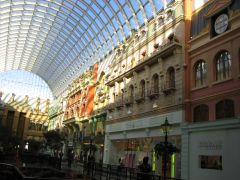
\includegraphics[width=.45\linewidth]{gfx/example_1}} \quad
% \subfloat[Pan ma signo.]
% {\label{fig:example-b}
% 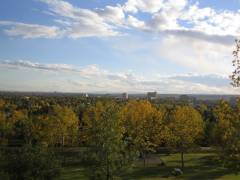
\includegraphics[width=.45\linewidth]{gfx/example_2}} \\
% \subfloat[Methodicamente o uno.]
% {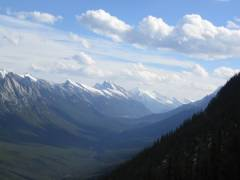
\includegraphics[width=.45\linewidth]{gfx/example_3}} \quad
% \subfloat[Titulo debitas.]
% {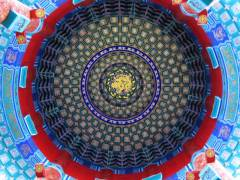
\includegraphics[width=.45\linewidth]{gfx/example_4}}
% \caption[Tu duo titulo debitas latente]{Tu duo titulo debitas latente.}\label{fig:example}
% \end{figure} % Chapter 2
% % Chapter 3

\chapter{Math Test Chapter} % Chapter title

\label{ch:mathtest} % For referencing the chapter elsewhere, use \autoref{ch:mathtest}

%----------------------------------------------------------------------------------------

\lipsum[13]

%----------------------------------------------------------------------------------------

\section{Some Formulas}

Due to the statistical nature of ionisation energy loss, large fluctuations can occur in the amount of energy deposited by a particle traversing an absorber element\footnote{Examples taken from Walter Schmidt's great gallery: \\ \url{http://home.vrweb.de/~was/mathfonts.html}}.  Continuous processes such as multiple scattering and energy loss play a relevant role in the longitudinal and lateral development of electromagnetic and hadronic showers, and in the case of sampling calorimeters the measured resolution can be significantly affected by such fluctuations in their active layers.  The description of ionisation fluctuations is characterised by the significance parameter $\kappa$, which is proportional to the ratio of mean energy loss to the maximum allowed energy transfer in a single collision with an atomic electron: \graffito{You might get unexpected results using math in chapter or section heads. Consider the \texttt{pdfspacing} option.}
\begin{equation}
\kappa =\frac{\xi}{E_{\mathrm{max}}} %\mathbb{ZNR}
\end{equation}
$E_{\mathrm{max}}$ is the maximum transferable energy in a single collision with an atomic electron.
\[E_{\mathrm{max}} =\frac{2 m_{\mathrm{e}} \beta^2\gamma^2 }{1 + 2\gamma m_{\mathrm{e}}/m_{\mathrm{x}} + \left ( m_{\mathrm{e}} /m_{\mathrm{x}}\right)^2}\ ,\]
where $\gamma = E/m_{\mathrm{x}}$, $E$ is energy and $m_{\mathrm{x}}$ the mass of the incident particle, $\beta^2 = 1 - 1/\gamma^2$ and $m_{\mathrm{e}}$ is the electron mass. $\xi$ comes from the Rutherford scattering cross section and is defined as:
\begin{eqnarray*} \xi  = \frac{2\pi z^2 e^4 N_{\mathrm{Av}} Z \rho
\delta x}{m_{\mathrm{e}} \beta^2 c^2 A} =  153.4 \frac{z^2}{\beta^2}
\frac{Z}{A}
\rho \delta x \quad\mathrm{keV},
\end{eqnarray*}
where

\begin{tabular}{ll}
$z$ & charge of the incident particle \\
$N_{\mathrm{Av}}$ & Avogadro's number \\
$Z$ & atomic number of the material \\
$A$ & atomic weight of the material \\
$\rho$ & density \\
$ \delta x$ & thickness of the material \\
\end{tabular}

$\kappa$ measures the contribution of the collisions with energy transfer close to $E_{\mathrm{max}}$.  For a given absorber, $\kappa$ tends towards large values if $\delta x$ is large and/or if $\beta$ is small.  Likewise, $\kappa$ tends towards zero if $\delta x $ is small and/or if $\beta$ approaches $1$.

The value of $\kappa$ distinguishes two regimes which occur in the description of ionisation fluctuations:

\begin{enumerate}
\item A large number of collisions involving the loss of all or most of the incident particle energy during the traversal of an absorber.

As the total energy transfer is composed of a multitude of small energy losses, we can apply the central limit theorem and describe the fluctuations by a Gaussian distribution. This case is applicable to non-relativistic particles and is described by the inequality $\kappa > 10 $ (\ie, when the mean energy loss in the absorber is greater than the maximum energy transfer in a single collision).

\item Particles traversing thin counters and incident electrons under any conditions.

The relevant inequalities and distributions are $ 0.01 < \kappa < 10 $, Vavilov distribution, and $\kappa < 0.01 $, Landau distribution.
\end{enumerate}

%----------------------------------------------------------------------------------------

\section{Various Mathematical Examples}

If $n > 2$, the identity \[t[u_1,\dots,u_n] = t\bigl[t[u_1,\dots,u_{n_1}], t[u_2,\dots,u_n] \bigr]\] defines $t[u_1,\dots,u_n]$ recursively, and it can be shown that the alternative definition \[t[u_1,\dots,u_n] = t\bigl[t[u_1,u_2],\dots,t[u_{n-1},u_n]\bigr]\] gives the same result. % Chapter 3
%% Chapter X

\chapter{Chapter Title} % Chapter title

\label{ch:name} % For referencing the chapter elsewhere, use \autoref{ch:name} 

%----------------------------------------------------------------------------------------

\section{Section Title}

Content

%------------------------------------------------

\subsection{Subsection Title}

Content

%------------------------------------------------

\subsection{Subsection Title}

Content

%----------------------------------------------------------------------------------------

\section{Section Title}

Content % Chapter 4 - empty template

%----------------------------------------------------------------------------------------
%	THESIS CONTENT - APPENDICES
%----------------------------------------------------------------------------------------

% \appendix

% % \part{Appendix} % New part of the thesis for the appendix

% % Appendix A

\chapter{Appendix Test}

%----------------------------------------------------------------------------------------

\lipsum[13-14]

%----------------------------------------------------------------------------------------

\section{Appendix Section Test}
\lipsum[15]

\graffito{More dummy text}
\lipsum[16]

%----------------------------------------------------------------------------------------

\section{Another Appendix Section Test}
\lipsum[17]

\begin{table}
\myfloatalign
\begin{tabularx}{\textwidth}{Xll} \toprule
\tableheadline{labitur bonorum pri no} & \tableheadline{que vista}
& \tableheadline{human} \\ \midrule
fastidii ea ius & germano &  demonstratea \\
suscipit instructior & titulo & personas \\
\midrule
quaestio philosophia & facto & demonstrated \\
\bottomrule
\end{tabularx}
\caption[Autem usu id]{Autem usu id.}
\label{tab:moreexample}
\end{table}

\lipsum[18]

\begin{lstlisting}[float,caption=A floating example]
for i:=maxint to 0 do
begin
{ do nothing }
end;
\end{lstlisting} % Appendix A
%% Appendix X

\chapter{Appendix Title}

%----------------------------------------------------------------------------------------

% Content begins here % Appendix B - empty template

%----------------------------------------------------------------------------------------
%	POST-CONTENT THESIS PAGES
%----------------------------------------------------------------------------------------

  \begin{thebibliography}{1}

  \bibitem{church} N Goodman, V Mansinghka, D Roy, K Bonawitz {\em Church: a language for generative models}  2012.

  \bibitem{paige}  RA Paige, O Danvy {\em Automatic program development: A tribute to Robert Paige} 2008:

  \bibitem{freer} CE Freer, DM Roy, JB Tenenbaum {\em Towards common-sense reasoning via conditional simulation: legacies of Turing in Artificial Intelligence} 2012 Arxiv:

  \bibitem{turing} A Turing {\em On computable numbers, with an application to the Entscheidungsproblem} 1936: Proceedings of the London mathematical society.

  \end{thebibliography}
% \cleardoublepage% Bibliography

\label{app:bibliography} % Reference the bibliography elsewhere with \autoref{app:bibliography}

\manualmark
\markboth{\spacedlowsmallcaps{\bibname}}{\spacedlowsmallcaps{\bibname}} 
\refstepcounter{dummy}

\addtocontents{toc}{\protect\vspace{\beforebibskip}} % Place the bibliography slightly below the rest of the document content in the table of contents
\addcontentsline{toc}{chapter}{\tocEntry{\bibname}}

\bibliographystyle{plainnat}

\bibliography{Bibliography} % Bibliography

% \cleardoublepage% Colophon (a brief description of publication or production notes relevant to the edition)

\pagestyle{empty}

\hfill

\vfill

\pdfbookmark[0]{Colophon}{colophon}

\section*{Colophon}

This document was typeset using the typographical look-and-feel \texttt{classicthesis} developed by Andr\'e Miede. The style was inspired by Robert Bringhurst's seminal book on typography ``\emph{The Elements of Typographic Style}''. \texttt{classicthesis} is available for both \LaTeX\ and \mLyX: 

\begin{center}
\url{http://code.google.com/p/classicthesis/}
\end{center}

\noindent Happy users of \texttt{classicthesis} usually send a real postcard to the author, a collection of postcards received so far is featured here: 

\begin{center}
\url{http://postcards.miede.de/}
\end{center}
 
\bigskip

\noindent\finalVersionString % Colophon

% \cleardoublepage% Declaration

\refstepcounter{dummy}
\pdfbookmark[0]{Declaration}{declaration} % Bookmark name visible in a PDF viewer

\chapter*{Declaration} % Declaration section text

\thispagestyle{empty}

Put your declaration here.
\bigskip
 
\noindent\textit{\myLocation, \myTime}

\smallskip

\begin{flushright}
\begin{tabular}{m{5cm}}
\\ \hline
\centering\myName, \today \\
\end{tabular}
\end{flushright}
 % Declaration

%----------------------------------------------------------------------------------------

\end{document}
